\chapter{Решение проблемы возврата регенерированного урана в топливный цикл}

\section{Разработка схем полного возврата}\label{sec:ch2/sec3}
\subsection{Модифицированный двойной каскад}

В качестве модификации двойного каскада была предложена альтернативная каскадная схема, которая позволяет обеспечить возврат регенерата в цикл в требуемом соотношении. В этой схеме, изображенной 
на рисунке \ref{fig:vestnik}, первая часть (каскад 1) увеличивает 
концентрацию $^{235}$U со всеми более легкими изотопами ($^{232}$U и $^{234}$U) и направляет их на вход второго каскада, который, в свою очередь, в легкой фракции будет концентрировать эти четные миноры в потоке загрязненного продукта \cite{smirnovObogashchenieRegenerirovannogoUrana2018}.
Изотопный же состав получаемый на выходе тяжелой фракции второго каскада, разбавляется НОУ-разбавителем, приготовленным из материала, не содержащего четных искусственных изотопов (ранее не облучаемого в реакторе) -- природного или обедненного урана -- для контроля концентраций $^{232}$U и $^{234}$U в допустимых пределах и для управления соотношением рециклируемых материалов (для поддержания соотношения регенерата в питании каскада к нарабатываемому продукту на требуемом уровне, который формально соответствует эквивалентному возврату (1:1) выгоревшего топлива в ядерный топливный цикл).

\begin{figure}[ht]
  \centerfloat{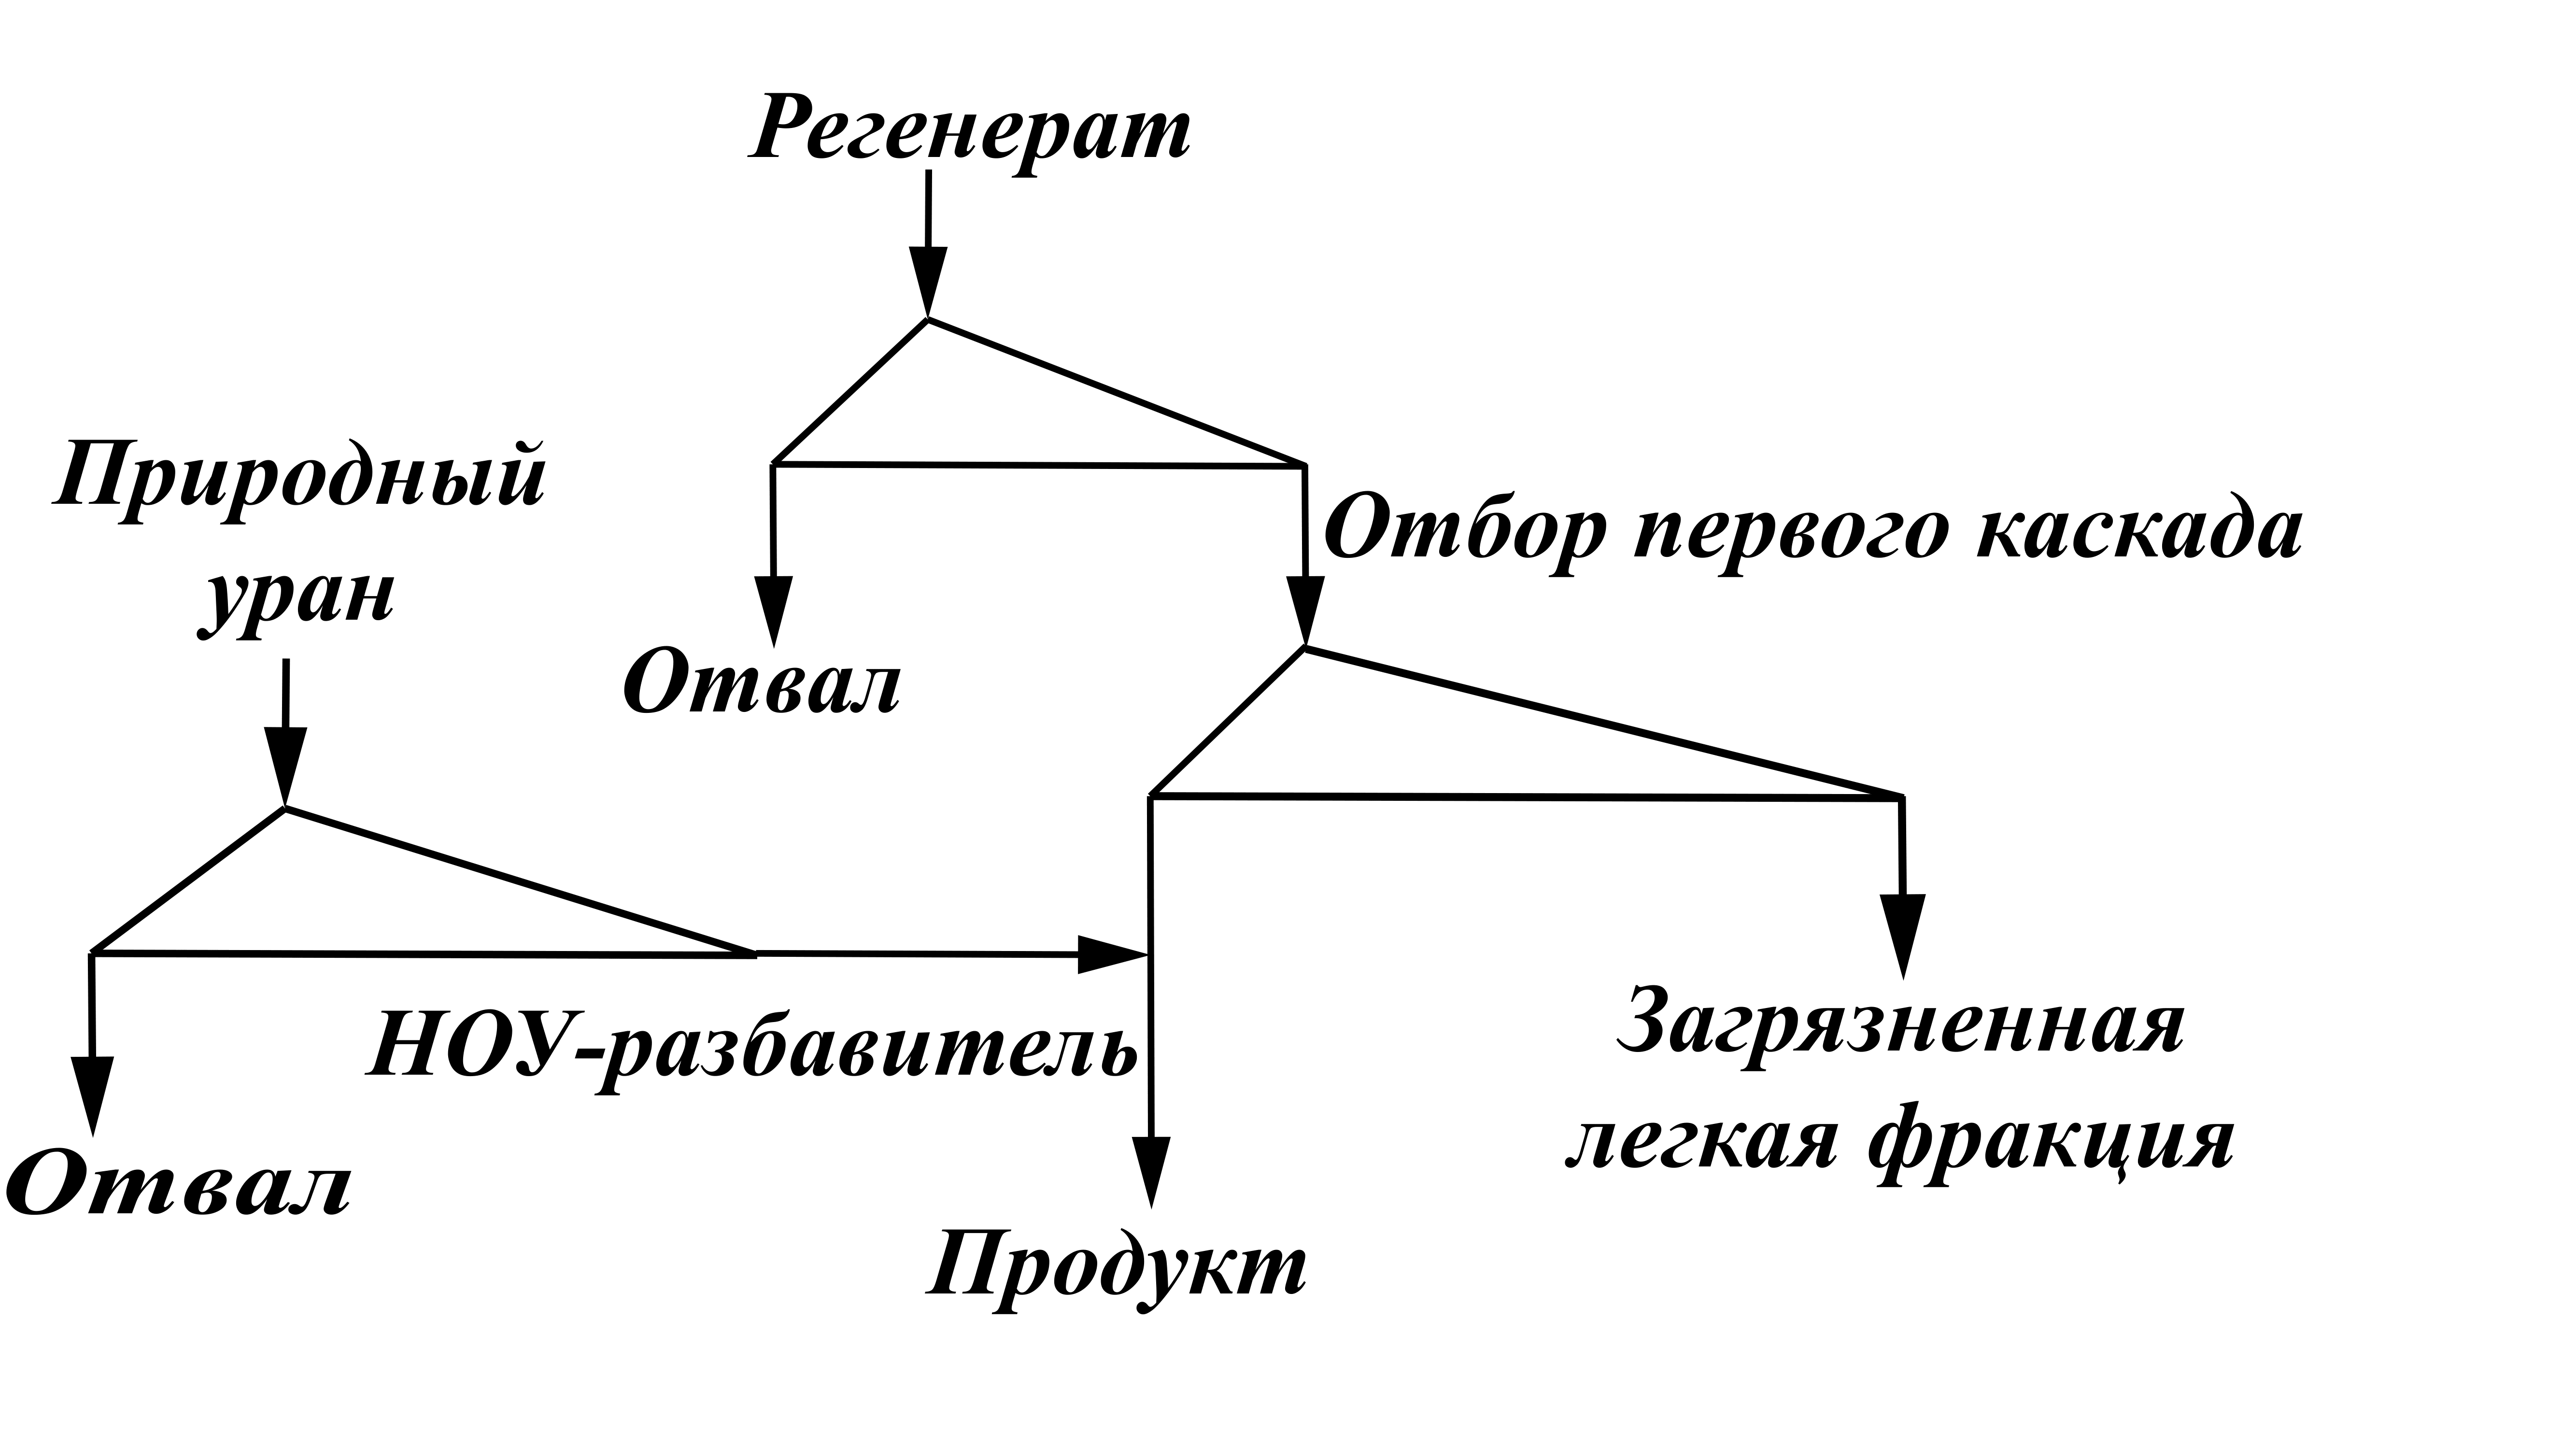
\includegraphics[scale=0.08]{cascades/triple}}
  \caption{Двойной каскад с добавлением НОУ (тройной каскад)}\label{fig:vestnik}
\end{figure}

Отличие предлагаемой схемы от двойного каскада (рис. \ref{fig:double_ru}) состоит в том, что поток отвала второго каскада не является конечным продуктом.
Финальным шагом получения товарного продукта является разбавление этого потока сырьём, не содержащим искусственных изотопов урана с целью их разбавления и, соответственно, обеспечения заданных ограничений по $^{232,236}$U.
Для выполнения условия полного возврата регенерата в цикл, отношение потоков НОУ-разбавителя и отвала второго каскада, которые образуют товарный продукт, является предопределённым, поскольку при заданной концентрации выходящих потоков обоих каскадов известным является отношение потока тяжелой фракции второго каскада к питающему регенерату, и при этом условиями задачи предопределено отношение потока исходного регенерата к конечному-НОУ.
В этом случае единственным параметром, позволяющим влиять на концентрацию $^{235}$U в товарном продукте, является концентрация данного изотопа в разбавителе (в потоке НОУ-разбавитель на рис. \ref{fig:vestnik}).
Таким образом, величину обогащения $^{235}$U в потоке этого разбавителя подбирают для конкретных заданных внешних условий \cite{smirnovObogashchenieRegenerirovannogoUrana2018}.

Очевидно, что, поскольку питанием первого каскада является исходный регенерат, а питанием второго -- полученный из него среднеобогащённый регенерат, то поток тяжёлой фракции на выходе из второго каскада будет по величине в несколько раз меньше, чем исходный поток регенерата. Такая работа каскада обеспечивает перерасход регенерата на единицу продукта. Следовательно, поток разбавителя должен в несколько раз превосходить по величине поток тяжелой фракции второго каскада. Однако, если в качестве разбавителя использовать, например, природный уран, это условие может привести к снижению концентрации $^{235}$U ниже требуемой величины. Если же в качестве разбавителя использовать низкообогащённый уран, то можно увеличить отношение потоков НОУ-разбавителя к <<отвалу>> второго каскада, доведя ее до требуемого значения.  
Такая схема близка к описанной в патенте \cite{zhurinSposobIzotopnogoVosstanovleniya2010}. Однако отличием предлагаемого двойного каскада является то, что ни в одном из каскадов в схеме не происходит превышение концентрации $^{235}$U выше значения 20\%. При этом в схеме  \cite{zhurinSposobIzotopnogoVosstanovleniya2010} концентрация $^{235}$U в потоке P1 достигает 90\% и более. Кроме того, величина отношения потока регенерата к конечному продукту на рис. \ref{fig:vestnik} всегда является строго заданной, что позволяет расходовать на получение заданного количества продукта требуемое количество регенерированного урана.

Итак, согласно \cite{smirnovObogashchenieRegenerirovannogoUrana2018} схема, представленная на рис. \ref{fig:vestnik}, позволяет обогатить регенерированный уран, полученный после пяти рециклов в топливе реакторов ВВЭР-1000 при соотношении расхода регенерата и продукта 0,93 и ограничении на концентрацию $^{232}$U соответствующему значению $5\cdot10^{-7}$\%. Представляет интерес анализ возможности обогащения регенерата в такой схеме при заданном соотношении между массами исходного регенерата и продукта больше единицы. Такое заданное условие моделирует ситуацию обогащения и вовлечения в воспроизводство топлива регенерированного урана, накопленного к текущему моменту за период эксплуатации легководных реакторов. Дополнительный интерес представляет анализ поведения характеристик подобной схемы в зависимости от ограничений на концентрацию изотопа $^{232}$U в продукте. 





Таким образом, использование модифицированного двойного каскада с добавленным потоком НОУ-разбавителя для перемешивания с одним из выходящих потоков второго каскада позволяет успешно обогащать многократно рециклированный уран с максимальным возвратом его в воспроизводство при различных ограничениях на концентрацию изотопа $^{232}$U в продукте, включая более строгие ограничения, чем приняты в настоящее время на заводах по фабрикации топлива для реакторов на тепловых нейтронах.

Хотя этот вариант каскада (рис. \ref{fig:vestnik}) и кажется идеальным, цена хранения побочного продукта из загрязненной смеси может быть неприемлемо высока, что мгновенно сделает схему нежизнеспособной, если нет способов избежать такого негативного побочного эффекта.

\subsection{Тройной каскад}
Итак, в прошлом подразделе, в качестве необходимой модификации двойного каскада была предложена схема каскада рис. \ref{fig:vestnik}, которая позволяет решить проблему возврата необходимого количества регенерата в цикл.

Хотя этот вариант и кажется подходящим для решения поставленной задачи, остается нерешенной судьба легкой фракции второго каскада из-за того, что хранение загрязненного побочного продукта может быть сопряжено с существенными дополнительными затратами, поэтому важен поиск способов избежать накопления этого материала.
Исходя из этого, в диссертационной работе предложено применить дополнительный каскад для утилизации потока загрязненной фракции.

Далее будет предложен краткий обзор такой каскадной схемы.
 
Итак, в \cite{smirnovMethodEnrichReprocessed2019}  было предложено применять дополнительный каскад для производства НОУ из загрязненной смеси, сильно разбавленной обедненным ураном (которые имеют высокую концентрацию $^{235}$U около $\approx$20\%), чтобы получить конечный продукт в двух исходящих потоках и достичь значительной экономии природного урана ($\approx$38\%) даже для <<грязной>> композиции, которая уже была пятикратно рециклирована (рис. \ref{fig:Tomsk}). Расчеты показали, что такой подход позволяет производить НОУ коммерческого качества, расходуя определенное количество переработанного урана и отвечая стандартным спецификациям для  $^{232}$U (и условиям, установленным для других четных изотопов). В то же время, предлагаемая схема обеспечивает большую экономию природного урана, чем большинство схем обогащения переработанного урана. Это могло бы также обеспечить широкомасштабную <<мобилизацию>> обедненного урана.

\begin{figure}[ht]
  \centerfloat{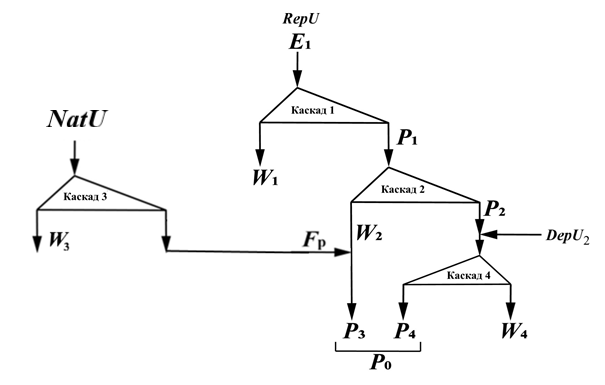
\includegraphics[scale=0.9]{cascades/triple_t}}
  \caption{Тройной каскад с подмешиванием ОГФУ и НОУ-разбавителем}\label{fig:Tomsk}
\end{figure}

Схема такого каскада, состоящего из четырех ординарных каскадов, решает проблему обращения с легкой фракцией, вышедшей из второго каскада.
Это позволяет вовлечь больше $^{235}$U, и избавляет от необходимости конечной утилизации материала с высоким содержанием $^{232}$U.
Принцип работы такой схемы состоит в следующем.
Теперь финальный продукт -- низкообогащенный уран -- получается путем смешения двух потоков.
Первый из них аналогичен финальному продукту, полученному посредством двойного модифицированного каскада.
Второй же нарабатывается из загрязненной смеси, сильно разбавленной обедненным ураном.
При этом, конфигурация подбирается таким образом, чтобы на получение единицы продукта из этих совмещенных потоков затрачивалось требуемое количество ($\approx$0.93) питающего регенерата.

Итак, данная схема позволяет получить конечный НОУ-продукт требуемого качества, смешав два производящих потока и достичь значительной экономии природного урана ($\approx$38\%) даже для «грязного» регенерата, который уже  пятикратно был рециклирован.
При этом, для того же исходного состава регенерата, схема двойного модифицированного каскада (рис. \ref{fig:vestnik}) показывает лишь ($\approx$8\%) в сокращении расхода природного урана в сравнении с ординарным, обогащающим природный уран \cite{smirnovObogashchenieRegenerirovannogoUrana2018}.
Однако, такой эффект связан с двухкратным перерасходом работы разделения в схеме тройного каскада, тогда как в схеме двойного модифицированного каскада затрачивается лишь ($\approx$13\%) дополнительной работы разделения.
Это связано с большим объемом вовлечения ОГФУ для разбавления загрязненного потока легкой фракции второго каскада.
Расчеты показали, что такой подход позволяет производить НОУ коммерческого качества, расходуя должное количество переработанного урана, в то же время отвечая стандартным спецификациям $^{232}$U (и условиям, установленным для других четных изотопов).
В то же время, предлагаемая схема обеспечивает более существенную экономию природного урана, чем большинство схем обогащения регенерированного урана.
Такая схема позволяет также обеспечить широкомасштабную «мобилизацию» обедненного урана.

\section{Сравнение схем полного возврата}

Чтобы проиллюстрировать преимущества и недостатки различных рассмотренных ранее схем, предназначенных для возврата регенерированного урана в ЯТЦ, в данной части диссертационной работы проводится их сравнительный анализ, помогающий сделать предварительные технико-экономические оценки.
Для этого, ключевые характеристики, связанные с общей эффективностью, такие как экономия природного урана, расход работы разделения и энергозатраты, были оценены для каждой схемы в удельных единицах (на единицу продукции).
Затем они были нормированы на величины, характерные для ординарного каскада(трехпоточного).
Чтобы избежать стоимостных показателей затрат, была использована методология пересчета ключевых показателей (экономия природного урана, объем обогащаемого ОГФУ и затраты работы разделения) в единицы потребляемой энергии (мегаватт-часы)  \cite{rodionovaAnalizTehnikoekonomicheskihHarakteristik2019}.
Этот показатель и был предложен в качестве универсального инструмента оценки рассматриваемых каскадов, используемых для повторного обогащения урана.

Концентрация $^{235}$U в потоках отбора второго каскада ограничена уровнем 19,99\% (чтобы не превышать пороговое значение концентрации $^{235}$U для низкообогащенного урана). Для каждого каскада с индексом 2 опорный компонент составляет $^{236}$U и $^{238}$U -- для остальных каскадов.

В качестве схемы №1 рассматривается двойной каскад (рис. \ref{fig:double_ru}), в качестве схемы №2 -- двойной модифицированный (рис. \ref{fig:vestnik}), а в качестве схемы №3 -- тройной каскад (рис. \ref{fig:Tomsk}), для которого подбирается уровень перерасхода работы разделения на уровне 25\% и 50\%, относительно ординарного каскада, обогащающего природный уран для аналогичных значений $^{235}$U.
\begin{table}[h]
  \begin{center}
  \begin{tabular}{|c|c|c|c|c|c|}
  \hline
  \makecell{Схема, №} & \makecell{Экономия  \\ природного  \\ урана,\% }
  & \makecell{Перерасход \\ работы  \\ разделения, \%}
  & \makecell{Расход  \\ регенерата  \\ на единицу \\  продукта}
  & \makecell{Расход  \\ ОГФУ \\  на  \\ единицу \\  продукта} & \makecell{Относительная  \\ стоимость, \%} \\
  \hline
  1&100&41.63&8.26&0&0.32\\
  2&10.07&6.08&0.93&0&89.96\\
  3&15.08&25&0.93&31.11&85.00\\
  3&23.13&50&0.93&74.49&77.02\\
  \hline
  \end{tabular}\caption{Интегральная таблица характеристик сопоставляемых каскадных схем.}\label{4comp}
  \end{center}
\end{table}

Несмотря на 100\% экономию природного урана и, следовательно, низкую относительную стоимость, схема №1  -- двойной каскад -- (рис. \Ref{fig:double}) не соответствует требованиям к содержанию $^{232}$U в конечном продукте.\\
Поэтому результаты, которые показывают, что выигрыш в экономии природного урана (и, как следствие, в относительной себестоимости) обусловлен лишь незначительным дополнительным расходом работы разделения, не могут считаться удовлетворительными.
Рассмотренные схемы, кроме №1, производили НОУ заданного реакторного качества, обеспечивая при этом требуемую пропорцию расхода регенерата на единицу продукта.
Схемы же №3и №4 (рис. \ref{fig:vestnik},\ref{fig:Tomsk}) могут обеспечить желаемое соотношение потребления регенерата на единицу продукта, а №4 (рис. \ref{fig:Tomsk}) демонстрирует наилучшие результаты в сохранении природного урана, которые могут быть еще увеличены с помощью дополнительной работы разделения (с более полным извлечением $^{235}$U при удлинении обеднительных частей каскадов).
И, как ранее было отмечено, схема №4 является единственной схемой из рассмотренных, которая предотвращает накопление токсичных отходов (изотопный состав с высоким содержанием $^{232}$U и $^{235}$U).
Однако, сопутствующая <<мобилизация>> обедненного урана хоть и может иметь дополнительные преимущества, поскольку складские запасы этого материала сами по себе являются проблемой, она требует дополнительных затрат работы разделения\cite{fitchOPTIONSDISPOSALREAPPLICATION2009}.
При рассмотренном критерии себестоимости, соответствующим энергозатратам на единицу НОУ, увеличение разделительной работы сопровождается снижением себестоимости, так как сэкономленный уран вносит самый значительный вклад в изменение этого показателя \cite{gusevMultycascadeEnrichmentSchemes2020}. \\
Отсюда можно сделать вывод, что каскадная схема №4 (рис. \ref{fig:Tomsk}) являетсянаиболее предпочтительной для решения задачи возврата регенерата в ЯТЦ в многократном рецикле, в условиях, когда используется способ стоимостной оценки, отдающий предпочтение экономии природного урана.

Недостаток способа состоит в том, что такой подход хоть и позволяет на 100\% решить проблему с накоплением загрязненных $^{232}$U отходов, вынуждает использовать значительные объемы ОГФУ.

% Поэтому, в качестве альтернативы была предложена схема рисунка \ref{fig:patent}), в которой на каскад с индексом 3 подается смесь грязного потока легкой фракции каскада 2, которая разбавляется обедненным гексафторидом урана до содержания $^{235}$U на уровне природного урана. Этот поток в дальнейшем разбавляется чистым природным ураном, пропорция которого подбирается для выполнения всех заданных условий.
% \begin{figure}[ht]
%   \centerfloat{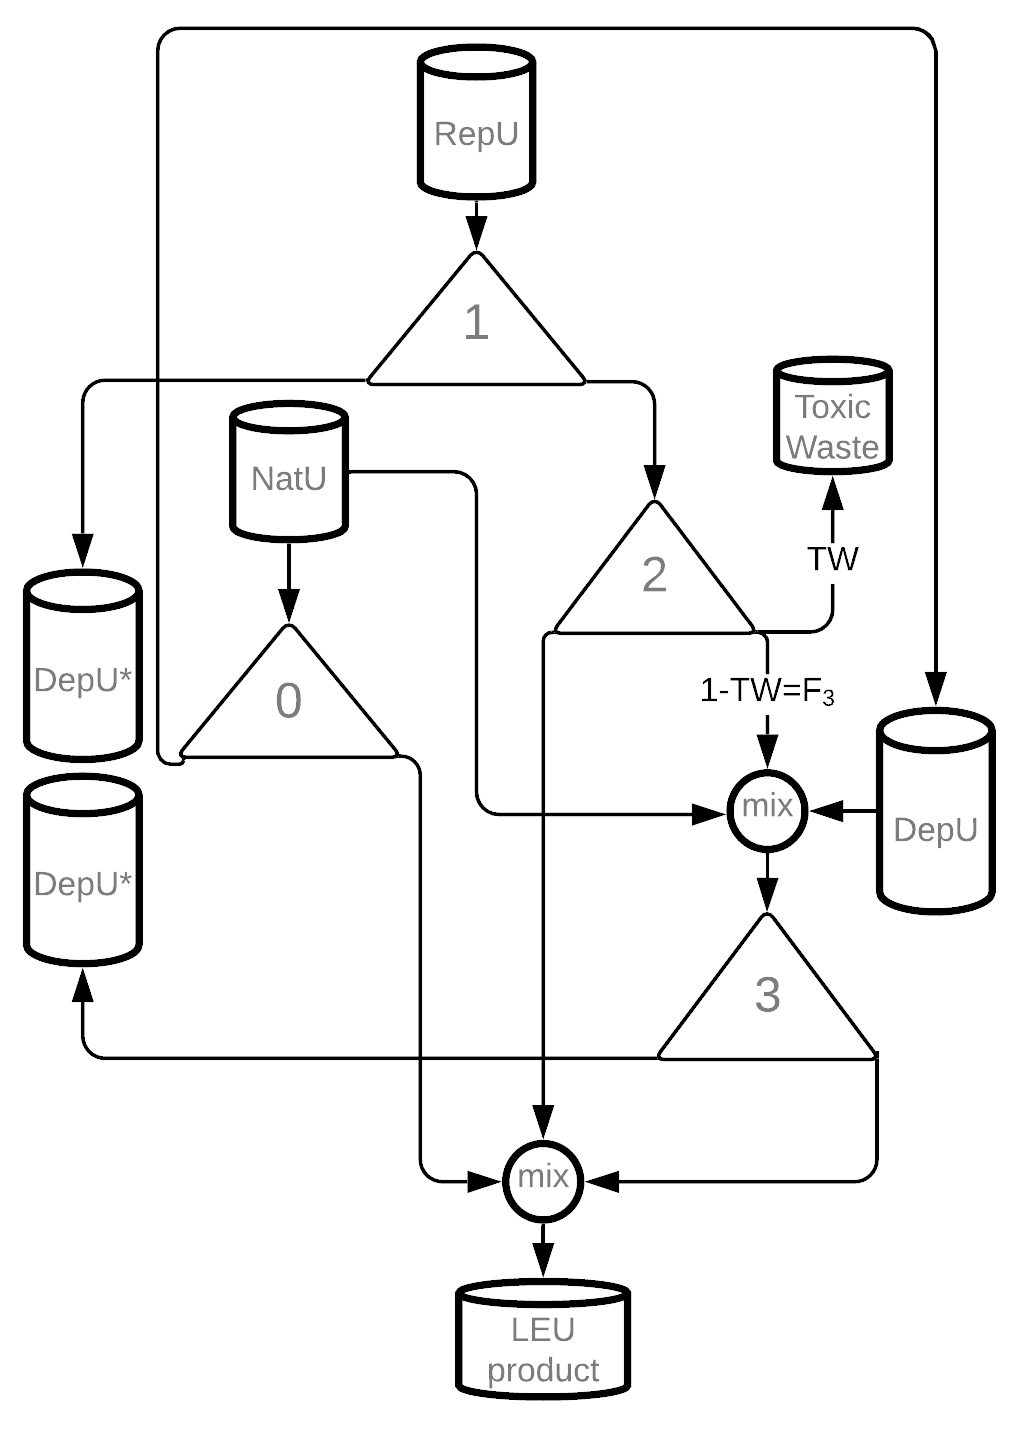
\includegraphics[scale=0.3]{cascades/triple_cascade_complete_return}}
%   \caption{Тройной каскад с подмешиванием НОУ, ОГФУ и природного урана}\label{fig:patent}
% \end{figure}

% Как мы видим, такие схемы также очень ценны как инструмент для переработки предписанного количества выделенного из ОЯТ урана.

Так как наиболее ценны схемы, которые решают вопрос включения побочной легкой фракции в производство свежего НОУ, в качестве альтернатив могут быть рассмотрены следующие схемы.

Одним из вариантов утилизации побочной легкой фракции, образующейся во втором каскаде схемы рис. \ref{fig:vestnik}, является возможность смешать этот побочный продукт с обедненным ураном и отправить на последующее длительное хранение \cite{vodolazskihSposobIzotopnogoVosstanovleniya}. Здесь поток легкой фракции второго каскада разбавляется обедненным гексафторидом из имеющихся складских запасов (дважды обедненным, с низким содержанием $^{235}$U $\approx$0,1\%), отправляя полученную ядерно-безопасную смесь на длительное хранение. Недостатки этого метода заключаются в том, что, хотя этот подход позволяет полностью решить проблему накопления загрязненных отходов $^{232}$U, он вынуждает использовать значительные объемы обедненного гексафторида (в $\approx$50 раз больше, чем разбавляемая им изотопная смесь), а также как тот факт, что значительная масса целевого изотопа $^{235}$U будет потеряна для возможности применения в производстве свежего НОУ, что снизит эффективность использования переработанного урана, которая выражается в степени извлечения $^{235}$U из регенерата. Степень извлечения этого изотопа для схемы двойного модифицированного каскада может быть записана как
$U^{235}_{Rec} = \frac{P \cdot C_{P}^{235}}{F_0 \cdot C_{NatU}^{235} + E \cdot C_{E}^{235}}$, где массовые потоки $P$, $E$ и $F_0$ умножены на концентрации $^{235}$U в этих потоках.

Тогда как в таком варианте предлагается избавиться от радиоактивного материала с высокой концентрацией $^{232}$U путем разбавления его обедненным гексафторидом и последующей отправкой на хранение, помимо методов, позволяющих избежать его накопления, применяя его для конечного производства НОУ, таких как тройные схемы \cite{smirnovMethodEnrichReprocessed2019}, существует вариант направить поток легкой фракции на питание другого двойного каскада, производящего НОУ для последующего цикла \cite{nevinicaToplivnyyCiklLegkovodnogo2019}. Такую схему  каскада целесообразно использовать в условиях многократного рецикла урана, начиная со второго рецикла, а также в условиях постоянного производства регенерированного топлива для парка реакторов на тепловых нейтронах. Устройство этой схемы, изображенной на рис. \ref{P2utilizationRing} предлагает вовлекать этот материал после его накопления в результате обогащения изначальной партии регенерата $E$, поступившей на обогатительное производство в обогащение следующей партии регенерированного урана $E'$ из переработанных ОТВС. Показано, что реализация предлагаемой схемы позволяет полностью израсходовать как вновь поступивший на повторное обогащение регенерированный уран, так и проблемный промежуточный продукт $P_2$, оставшийся после прошлой операции по дообогащению -- гексафторид высокообогащенного урана с относительно высоким содержанием $^{232}$U.

\begin{figure}[ht]
  \centerfloat{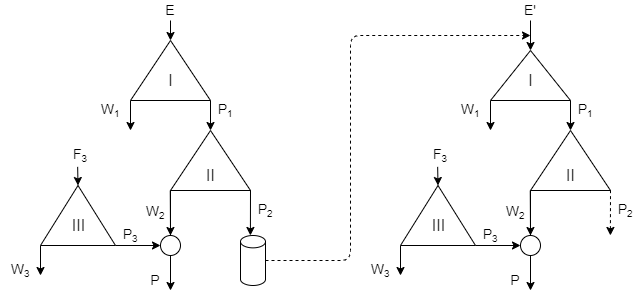
\includegraphics[scale=0.7]{cascades/P2utilizationRing}}
  \caption{Схема передачи загрязненной изотопом $^{232}$U фракции гексафторида урана в двойном каскаде от первой партии дообогащенного регенерированного урана к последующей.}\label{P2utilizationRing}
\end{figure}

Процесс возврата данного материала в воспроизводство низкообогащенного урана может быть начат практически после дообогащения регенерата уже для одной ТВС и даже для ее части (непрерывный возврат), схема каскада при этом преобразуется к виду, когда проблемный промежуточный продукт $P_2$ возвращается и подмешивается к потоку питающего исходного регенерата $E$.

Очевидно, что при использовании предлагаемой схемы и непрерывной работе завода по обогащению, удастся полностью замкнуть топливный цикл по урану, а единственным отходом производства станет только обедненный гексафторид, образующийся в отвале первого каскада. Однако данный продукт можно считать штатным отходом
обогатительного производства, для которого на сегодняшний день отработаны технологии хранения и переработки. При этом после вывода завода из эксплуатации (или остановки на планово-предупредительный ремонт) останется невостребованным только тот объем обогащенного по изотопу $^{232}$U гексафторида урана, который будет образован после обогащения последней партии регенерата на этом заводе. Таким образом, предлагаемый в настоящей статье подход к дообогащению регенерата урана позволяет организовать полный возврат регенерированного урана в топливный цикл в течение практически всего жизненного цикла топлива легководных реакторов,
работающих в замкнутом топливном цикле, как показывают результаты работы \cite{nevinicaToplivnyyCiklLegkovodnogo2019}.



\clearpage